\documentclass[11pt,onecolumn]{article}
\usepackage{pgfplots}
\usepackage{hyperref}% http://ctan.org/pkg/hyperref
\AtBeginDocument{%
  \let\oldref\ref% 
  \def\ref{\oldref*}}
\usepackage{amsmath}
\usepackage{amsthm}
\usepackage{amssymb}
\usepackage{bbold}
\usepackage[justification=centering]{caption}
\usepackage{lipsum}
\usepackage[width=.6\textwidth,format=plain,labelsep=period,justification=centerlast]{caption}
\usepackage[inner=2.5cm,outer=2cm, top=1.5cm, bottom=1.5cm]{geometry}
\pgfplotsset{ticks=none}
\tikzset{pointille/.style={dash pattern = on 2pt off 2pt on 6pt off 2pt}}
\tikzset{points/.style={dash pattern = on 1pt off 1pt}}
\tikzset{tirets/.style={dash pattern = on 5pt off 5pt}}
\newtheorem{theorem}{\textit{Theorem}}

\begin{document}
\title{A Report on the Ziggurat Method}
\author{Daniel de Souza Severo\\
Dept. of Electrical and Computer Engineering\\
University of Toronto}
\date{July, 2014}
\maketitle
\begin{abstract}

\textbf{This report outlines, as well as provides a mathematical proof of functionality, of a highly efficient pseudo-random number generator: The Ziggurat Method. A simple ready-to-use code has been provided by previous authors. We contribute to this with a speed test on a modern Intel processor, as well as a Python script that generates all the necessary information to implement a specific version of the algorithm.}
\end{abstract}

\section{Introduction}
Pseudo-random number generators (PRNG's) are crucial in the context of simulating noise in communication channels. We present a report on an efficient method for generating pseudo-random samples from any decreasing probability distribution called the Ziggurat Method. The initial idea was developed by \cite{marsaglia}, but has been enhanced by Marsaglia, Tsang \cite{marsaglia&tsang} and others. Specifically, we will show the latest and most efficient version presented by McFarland \cite{mcfarland}. In the latter paper, the method shows a speedup of over 3 times compared to traditional algorithms such as Marsaglia's Polar Method \cite{marsagliapolar}. We present a speed comparison in C implemented on an Intel i7-4790 clocked at 3.60 GHz. McFarland \cite{mcfarland} provides all the necessary code to implement an \textit{ad hoc} version of the algorithm, as well as a ready-to-use C code for a univariate Gaussian. A proof that the samples from this method are truly Gaussian is also provided.

\section{Uniform region sampling}\label{ugs}
Prior to explaining the method, a prelude into a simple, yet important, mathematical result in probability theory is due. Most pseudorandom number generators operate on the principle that sampling a point $x$ directly from the distribution in question, call it $g$, is equivalent to the following:
\begin{enumerate}
	\item Divide the region $A$ under $g$ into subregions $A_i$ such that $\{A_i, \dotsb, A_N\}$ is a partition\footnote{This means that $A=\bigcup_{i=1}^N A_i$ and $A_i \cap A_j=\emptyset$ for all $i\neq j$.} of $A$.
	\item Randomly select a region $A_i$ with probability proportional to it's area, $\mu(A_i)$.
	\item Uniformly sample a point $p=(x,y)$ from the selected region $A_i$.
	\item Return $x$, since it will have distribution $g$.
\end{enumerate}

The validity of this method can be simply proven. Let $I$ be a random variable with distribution $f_I(i)=\mu(A_i)/\mu(A)=\mu(A_i)$ that represents part 2. of the method presented above. If $P=(X,Y)$ represents the points uniformly sampled in each region, then $f_{P|I}(p|i)=\mathbb{1}\{p \in A_i\}/\mu(A_i)$.\footnote{$\mathbb{1}\{x\}=1$ if $x$ is true and $0$ if it is false.} We can now calculate $f_P(p)=f_{X,Y}(x,y)$:
$$f_P(p)=\sum_i f_{P,I}(p,i)=\sum_i f_I(i)f_{P|I}(p|i)=\sum_i \mu(A_i)\frac{\mathbb{1}\{p \in A_i\}}{\mu(A_i)}=\sum_i \mathbb{1}\{p \in A_i\}$$
A specific point $p$ can only belong to one subregion, since $A_i \cap A_j=\emptyset, \forall i\neq j$. Hence, we have that: 
$$f_P(p)=\sum_i \mathbb{1}\{p \in A_i\} = \mathbb{1}\{p \in A_1\} + \mathbb{1}\{p \in A_2\} + \dotsb + \mathbb{1}\{p \in A_N\} = 1$$
$$f_X(x)=\int_y f_{X,Y}(x,y)dy = \int_0^{g(x)}dy = g(x)$$
The Ziggurat Method takes advantage of this result, by partitioning the region under $g$ into subregions that are easier to sample from than $g$ itself. A dataset generated from this method will have distribution $g$ up to machine precision.

\section{The Ziggurat Method}
The Ziggurat method uses the result from section \ref{ugs} to quickly generate pseudorandom numbers from any decreasing distribution. The density in question, we will denote it as $g$, is partitioned into small rectangular layers of equal area such as in figure \ref{fig:zig}.

\begin{figure}[h]
\centering
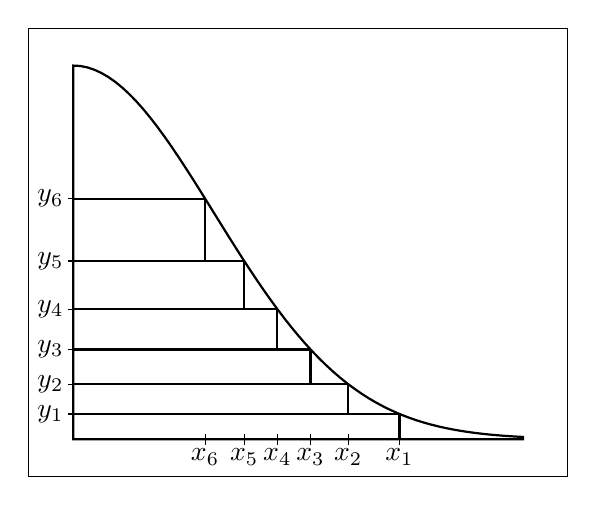
\begin{tikzpicture}
\begin{axis}[samples=65]    
 	\addplot[thick,domain=0:3.2] {2/sqrt(2*pi)*exp(-x^2/2)}\closedcycle;
 	\addplot [thick,color=black,mark=]coordinates {(2.3221253415052108722, 0.053829996928147945431) (0, 0.053829996928147945431)};
 	\addplot [thick,color=black,mark=]coordinates {(2.3221253415052108722, 0.053829996928147945431) (2.3221253415052108722, 0)};
 	
 	\addplot [thick,color=black,mark=]coordinates {(1.9563286553575721702, 0.11772519145881991813) (0, 0.11772519145881991813)};
 	\addplot [thick,color=black,mark=]coordinates {(1.9563286553575721702, 0.11772519145881991813) (1.9563286553575721702, 0.053829996928147945431)};
 	
	\addplot [thick,color=black,mark=]coordinates {(1.6886556366482920007, 0.19174857271380732284) (0, 0.19174857271380732284)};
 	\addplot [thick,color=black,mark=]coordinates {(1.6886556366482920007, 0.19174857271380732284) (1.6886556366482920007, 0.11772519145881991813)};
 	
	\addplot [thick,color=black,mark=]coordinates {(1.4526281686201162346, 0.27779949937230677675) (0, 0.27779949937230677675)};
 	\addplot [thick,color=black,mark=]coordinates {(1.4526281686201162346, 0.27779949937230677675) (1.4526281686201162346, 0.19174857271380732284)};	
 	
	\addplot [thick,color=black,mark=]coordinates {(1.2169036475136748573, 0.38051921777843910984) (0, 0.38051921777843910984)};
 	\addplot [thick,color=black,mark=]coordinates {(1.2169036475136748573, 0.38051921777843910984) (1.2169036475136748573, 0.27779949937230677675)};	 	
 	
 	\addplot [thick,color=black,mark=]coordinates {(0.93836855027265858619, 0.51372913829813168844) (0, 0.51372913829813168844)};
 	\addplot [thick,color=black,mark=]coordinates {(0.93836855027265858619, 0.51372913829813168844) (0.93836855027265858619, 0.38051921777843910984)};
 	
	\addplot [black, mark = -, nodes near coords=$y_6$,every node near coord/.style={anchor=0}] coordinates {(0, 0.51372913829813168844)};	
 	
 	\addplot [black, mark = -, nodes near coords=$y_5$,every node near coord/.style={anchor=0}] coordinates {(0, 0.38051921777843910984)};
 	
 	\addplot [black, mark = -, nodes near coords=$y_4$,every node near coord/.style={anchor=0}] coordinates {(0, 0.27779949937230677675)}; 	
 	\addplot [black, mark = -, nodes near coords=$y_3$,every node near coord/.style={anchor=0}] coordinates {(0, 0.19174857271380732284)};
 	
 	\addplot [black, mark = -, nodes near coords=$y_2$,every node near coord/.style={anchor=0}] coordinates {(0, 0.11772519145881991813)};
 	
	 \addplot [black, mark = -, nodes near coords=$y_1$,every node near coord/.style={anchor=0}] coordinates {(0, 0.053829996928147945431)}; 	
	 
	 \addplot [black, mark = |, nodes near coords=$x_6$,every node near coord/.style={anchor=90}] coordinates {(0.93836855027265858619, 0)};	
 	
 	\addplot [black, mark = |, nodes near coords=$x_5$,every node near coord/.style={anchor=90}] coordinates {(1.2169036475136748573, 0)};
 	
 	\addplot [black, mark = |, nodes near coords=$x_4$,every node near coord/.style={anchor=90}] coordinates {(1.4526281686201162346, 0)}; 	
 	\addplot [black, mark = |, nodes near coords=$x_3$,every node near coord/.style={anchor=90}] coordinates {(1.6886556366482920007, 0)};
 	
 	\addplot [black, mark = |, nodes near coords=$x_2$,every node near coord/.style={anchor=90}] coordinates {(1.9563286553575721702, 0)};
 	
	 \addplot [black, mark = |, nodes near coords=$x_1$,every node near coord/.style={anchor=90}] coordinates {(2.3221253415052108722, 0)}; 	
 	
 	
\end{axis}
\end{tikzpicture}
	\caption{Bins of the Ziggurat algorithm for area size equal to $1/8=0.125$ $(N=8)$. Only 6 bins can be inserted under the curve $(L_{max}=6)$, hence the layers occupy $0.75$ of the total area.}
	\label{fig:zig}
\end{figure}

Initially we must choose a number $N$ of layers each with area $1/N$. Given that the total area the layers occupy is equal to the area under $g$, we can not fit all of them under the curve $g$. We now define $L_{max}$ as the total number of layers that can be inserted under $g$. The leftover regions to the right of each layer, including the cap and tail of the distribution, now represent $1-L_{max}/N$ of the area under the distribution. 

In the light of section \ref{ugs}, we may now think of this problem as region sampling under a defined distribution $g$, with $L_{max}$ rectangular regions, $R_1, \dotsb, R_{L_{max}}$ and one residual region $A_R$ representing all regions that remain outside the rectangles, such that:
$$A_R=\bigcup_{i=1}^{L_{max}+1} A_i$$
where $A_i$ are the actual leftover regions (one for each rectangular region), cap included. The method then has 2 levels, first it randomly chooses to sample either from a layer or from the residual region. If a rectangular layer is chosen, it returns a uniform sample. If the residual region is select, it then must first randomly pick a leftover region to sample from. For these regions, with the exception of the tail, rejection sampling is applied (see Appendix \ref{rsampling}) to generate a uniform sample. If the tail is chosen, we use a fallback algorithm.

For the sake of illustration, we give an example for $N=256$. We will denote the borders of each rectangular layer as $x_i$, where the top layer (under the cap) is $x_{L_{max}+1}$ and the one that has the tail to the right of it is $x_1$. The area of each rectangle will be $1/256$. From simulations with the code provided in section \ref{implementation}. we know that $L_{max}=253$, so the total residual area will be $3/256$. We now do the following:
\begin{enumerate}
	\item Sample an integer $i$ uniformly between $1$ and $N=256$.
	\item If $i\in[1,L_{max}=253]$, return $x$ uniformly from region $[0,x_i)$. (This represents the layers).
	\item Else, sample an integer $j\in[1,254]$ with probability $p(j)=\mu(A_j)/\mu(A_R)$.
	\begin{enumerate}
		\item If $j=1$, return a sample $x$ from the tail.
		\item Else, apply Rejection Sampling to get a uniform sample $x$ from region $j$.
	\end{enumerate}
\end{enumerate}

To implement this method we require 3 look-up tables. One for the ziggurat lengths $x_i$ and heights $y_i=g(x_i)$, as well as the area of leftover regions $A_j$. We also need a uniform generator to output the values of $i$, $j$ and $x$.

Since each region is selected with probability proportional to it's area, the method will generate samples $x$ with distribution $g$, according to section \ref{ugs}.

\section{Implementation and Speed}\label{implementation}
McFarland \cite{mcfarland} has made available all the necessary codes to be used in C, Python and MATLAB. It can be found at \url{https://bitbucket.org/cdmcfarland/fast_prng}. We have also uploaded a Python script that generates all the necessary tables ($x_i$, $y_i=g(x_i)$ and $A_j$) for any given bin size $N$: \url{https://github.com/dsevero/A-Report-on-the-Ziggurat-Method/blob/master/ziggurat/generate_tables.py}.

The header file \textit{normal.h} that has been made available by \cite{mcfarland}, and 
is available at the hyperlink above, can be readily inserted into any C code. It provides 
a function \textit{normal\_setup()} that must be called to initialize the pseudo-random
number generator and \textit{normal()} can be used to sample numbers from a univariate
Gaussian distribution ($\mu=0$ and $\sigma^2=1$). The area of the bins used to generate this specific code was $1/256$.

With respect to speed, the Ziggurat algorithm implemented in C for $N=256$, is over 4 times faster than the tradition polar method \cite{marsaglia}, running on an Intel i7-4790 clocked at 3.60 GHz with 16 GB of RAM. Since \textit{normal()} generates a univariate Gaussian, we compared the speed of computing $\sigma*normal()+\mu$ (also in C) to the one of reapplying the Ziggurat algorithm to a $\mu$,$\sigma$ Gaussian. No significant performance improvements were seen. McFarland \cite{mcfarland} provides other speed comparisons in different programming languages.

\section{Appendix}
Here we present some useful results, with proofs, related to Rejection Sampling and hand-picked probability distributions. We assume that the reader is familiar with introductory level calculus and probability theory.

\subsection{Rejection Sampling}\label{rsampling}
 	
\begin{figure}[h]
\centering
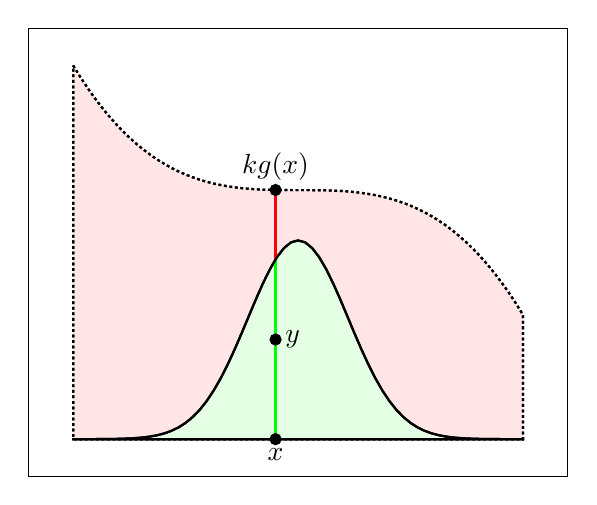
\begin{tikzpicture}
\begin{axis}[samples=65]    
 	\addplot[points,thick,domain=-1:1,fill=red!10] {0.25*(2-x^3)}\closedcycle;
 	\addplot[thick,domain=-1:1,fill=green!10] {1/(2*pi)^0.5*exp(-x^2/0.1)}\closedcycle;
    \addplot [thick,color=red,mark=]coordinates {(-0.1, 0.50025) (-0.1, 0)};
    \addplot [thick,color=green,mark=]coordinates {(-0.1, 0.36) (-0.1, 0)};
    \addplot[thick,domain=-1:1] {1/(2*pi)^0.5*exp(-x^2/0.1)}\closedcycle;
    \addplot[points,thick,domain=-1:1] {0.25*(2-x^3)}\closedcycle; \label{g_label}
	\addplot [black, mark = *, nodes near coords=$kg(x)$,every node near coord/.style={anchor=270}] coordinates {(-0.1, 0.50025)};
	\addplot [black, mark = *, nodes near coords=$y$,every node near coord/.style={anchor=180}] coordinates {(-0.1, 0.2)};
	\addplot [black, mark = *, nodes near coords=$x$,every node near coord/.style={anchor=90}] coordinates {(-0.1, 0)};
    \end{axis}
\end{tikzpicture}
	\caption{RSA rejection/acceptance regions. After sampling $x$ from $g$ (\ref{g_label}) if $y$ falls under curve $h$ (green) then it is stored, otherwise if it is above $h$ (red) it is rejected.}
	\label{fig:RSA}
\end{figure}

\begin{theorem}
Given two known distributions $g$ and $h$ defined over the same interval $A\subseteq\mathbb{R}$. We can create a dataset distributed according to $h$, by sampling only from $g$, if the following is done:

\begin{enumerate}
	\item Choose a number $k\in\mathbb{R^+}$ such that $kg(a)\geq h(a),\forall a\in A$.
	\item Sample a point $x$ from $g$.
	\item Sample a number $y$ from the distribution $Uniform[0,kg(x)]$.
	\item If $y<h(x)$ add it to the dataset, otherwise discard it.
\end{enumerate}
We will call this the \textit{Rejection Sampling Algorithm (RSA)}.
\end{theorem}

\begin{proof}
To show that the resulting dataset is distributed according to $h$, we may represent the sample points previously mentioned, $x$ and $y$, by the random variables $X \sim f_X(x)\equiv g(x)$ and $Y$, defined over a conditional distribution $f_{Y|X}(y|x)=Uniform[0,kg(x)]$, respectively. Also, define $Z=\mathbb{1}\{Y<h(X)\}$ such that if the sample $y$ is under the curve $h$, then $Z$ takes on the value $1$, otherwise $0$. Now, since $Y$ obeys a uniform distribution, we have that:

$$f_{Z|X}(z=1|x)=\frac{h(x)}{kg(x)}$$

Consider now the pair $(X,Z)$ where $(X,Z=1)$ represents the sample points $X$ that we will keep according to the RSA. Looking at the joint distribution: 
$$f_{X,Z}(x,z=1)=f_X(x)f_{Z|X}(z=1|x)=g(x)\frac{h(x)}{kg(x)}=\frac{1}{k}h(x)$$ 
we find that it distributes according to a multiple of $h(x)$, hence the dataset will have distribution $h$. 
\end{proof}

We may now discuss some interesting observations related to the Rejection Sampling Algorithm. Consider first the probability of keeping a generated value: $$f_Z(z=1)=\int_A f_{X,Z}(x,z=1)dx=\frac{1}{k}\int_A h(x)dx=\frac{1}{k}$$
Knowing this, it is interesting to define $k=\min_{\kappa\in\mathbb{R^+}}(\kappa g(a)\geq h(a), \forall a\in A)$, i.e. as the smallest $k\in\mathbb{R^+}$ such that $g$ is still above $h$. This way, we maximize the probability of keeping a generated value, thus minimizing computational efforts.\\

Let $P=(X,Y)$ be a random variable taking on values $p\in A\times [0,kg(x)]$, i.e. $P$ takes on values under curve $g$ (union of red and green regions of figure \ref{fig:RSA}). The joint distribution of $P$ is:
$$f_P(p)=f_{X,Y}(x,y)=f_X(x)f_{Y|X}(y|x)=g(x)\frac{1}{kg(x)}=\frac{1}{k}$$
from which we conclude that the RSA is equivalent to uniformly sampling points $(x,y)$ under $g$ and keeping only those that also fall under $h$. The $x$ coordinates of the stored points will have distribution $h$.

\subsection{Piecewise sampling}
Consider the following problem statement: given a distribution $g$, is it possible to divide $g$ into functions $g_1, ..., g_N$ such that sampling from these functions (in a specific way) is equivalent to sampling from $g$? Initially we will consider that $g=\sum_{i=1}^N g_i$ and we denote each region as $A_i\subseteq A$ as well as the area under each curve $g_i$ as $\pi_i$. Also the support of $g$ is $A=\bigcup_{i=1}^N A_i$.

\begin{figure}[h]
\centering
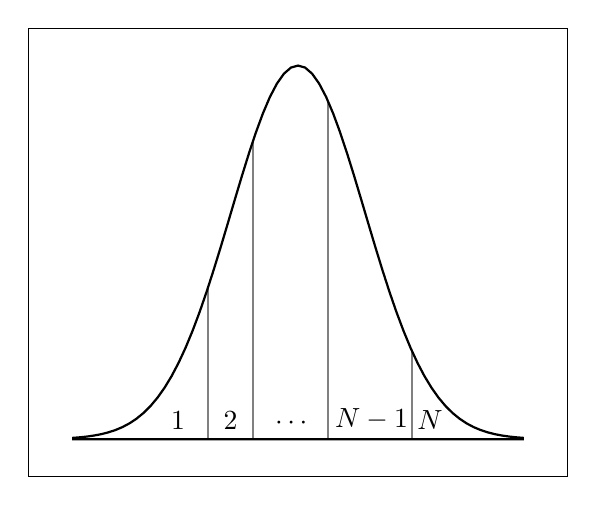
\begin{tikzpicture}
	\begin{axis}[samples=65]
	\addplot [thick,color=gray,mark=]coordinates {(-0.15, 0.31856) (-0.15, 0)};
	\addplot [thick,color=gray,mark=]coordinates {(-0.3, 0.16219) (-0.3, 0)};
	\addplot [thick,color=gray,mark=]coordinates {(0.1, 0.3609) (0.1, 0)};
	\addplot [thick,color=gray,mark=]coordinates {(0.38, 0.09414) (0.38, 0)};
 	\addplot[thick,domain=-0.75:0.75,] {1/(2*pi)^0.5*exp(-x^2/0.1)}\closedcycle;
 	\addplot [black, nodes near coords=$1$] coordinates {(-0.4, 0)};
 	\addplot [black, nodes near coords=$2$] coordinates {(-0.225, 0)};
 	\addplot [black, nodes near coords=$\dotsb$,every node near coord/.style={anchor=270}] coordinates {(-0.015, 0)};
 	 \addplot [black, nodes near coords=$N-1$] coordinates {(0.245, 0)};
 	\addplot [black, nodes near coords=$N$] coordinates {(0.44, 0)};
 	\end{axis}
\end{tikzpicture}
\caption{A general distribution $g$ being divided into $N$ regions, each with it's corresponding function $g_i$, region $A_i\subseteq A$ and area of region $\int_{A_i} g_i(x)dx=\pi_i$.}
\label{fig:psampling}
\end{figure}

We propose that the following algorithm solves the problem in question:
\begin{enumerate}
	\item Sample $\omega$ from $g$
	\item For $\omega\in A_i$, sample $x$ from $g_i/\pi_i$.
\end{enumerate}

If the above algorithm is followed, then $X$ will have distribution $g$. To prove that this is so, we define a random variable $Z$ taking on values $z\in\{1,\dotsb,N\}$ such that if $\omega\in A_i$ then $z=i$. In other words, $Z$ indicates to which region $\omega$ belongs to. Now, we know that:
$$f_Z(z)=P[\omega\in A_z]=\int_{A_z} g(x)dx=\int_{A_z} g_z(x)dx=\pi_z$$
Also, the joint distribution of $Z$ and $X$ is:
$$f_{Z,X}(z,x)=f_Z(z)f_{X|Z}(x|z)=\pi_z\frac{g_z(x)}{\pi_z}=g_z(x)$$
Since $X$ is what we are interested in, we now investigate it's distribution:
$$f_X(x)=\sum_z f_{Z,X}(z,x)=\sum_{z=1}^N g_z(x)=g(x)$$ 
This result shows that we may sample from the decompositions $g_1,\dotsb,g_N$ and still obtain a dataset with distribution $g$. Although this result is general, it says nothing of how it could be used to efficiently generate numbers from $g$ since part $1.$ of the algorithm requires that we sample from $g$ itself. This can be solved by considering the particular case in which the areas $\pi_i$ all have the same value. This area can be trivially calculated in the following way: since $g$ is a distribution we know that:
$$\int_A g(x)dx=\int_A \sum_{i=1}^N g_i(x)dx=\sum_{i=1}^N \int_{A_i} g_i(x)dx=N\int_{A_i} g_i(x)dx=1$$
$$\int_{A_i} g_i(x)dx=\frac{1}{N}$$
Since each region now has equal area, sampling $y$ from $g$ and checking the region in which $y$ has fallen into is equivalent to randomly generating an integer from the set $\{1,\dotsb,N\}$ and using it as $z$. We can now rewrite the original algorithm as:
\begin{enumerate}
	\item Sample $z$ uniformly from $\{1,\dotsb,N\}$.
	\item Sample $x$ from $Ng_z$
\end{enumerate}
The formal verification of this algorithm is straightforward:
$$f_Z(z)=\frac{1}{N}$$
$$f_{X|Z}(x|z)=Ng_z(x)$$
$$f_X(x)=\sum_z f_{X,Z}(x,z) = \sum_z f_Z(z)f_{X|Z}(x|z)=\sum_z \frac{1}{N}Ng_z(x)=g(x)$$
This result is useful as long as it is easier to sample from $g_1,\dotsb,g_N$ than it is from $g$. The Ziggurat method takes advantage of this and the fact that very efficient uniform pseudorandom number generators are available in most programming languages to create a simple algorithm to quickly generate samples from any decreasing density \cite{marsaglia&tsang}.



\newpage
\begin{thebibliography}{9}

\bibitem{marsaglia}
	George Marsaglia, "A convenient method for generating normal variables.", SIAM Rev. 6, 260-264, 1964.

\bibitem{marsagliapolar}
	George Marsaglia, Wai Wan Tsang, "A fast, easily implemented method for sampling from decreasing or symmetric unimodal density functions", SIAM Journ. Scient. and Statis. Computing, 5, 349-359, 1984.
	
\bibitem{marsaglia&tsang}
	George Marsaglia, Wai Wan Tsang, "The Ziggurat Method for Generating Random Variables", Journal of Statistical Software, 2000.

\bibitem{mcfarland}
	Christopher D. McFarland, "A modified ziggurat algorithm for generating exponentially- and normally-distributed pseudorandom numbers.", Apr. 2014.

\end{thebibliography}
\end{document}
